\chapter{Implementation} \label{Chapter:Implementation}

\section{Used software}

I started working on the prototype as soon as the initial designs and concepts have been written down. GitHub Projects\cite{gitHub} was used as a Kanban board to keep track of the tasks defined in \ref{section:Moscow}. The development was not split into multiple sprints, but it was rather following the waterfall method with the addition of continuous adaptation to changing requirements.

The latest version of Godot .NET (which at the time of starting the project was 4.3) was chosen as the game engine, thus the game was written in C\#. Rider, an IDE (Integrated Development Environment) made by JetBrains exclusively for .NET, was used as an external code editor. 

Three different software products were tried and used for the graphic assets. The most frequently used was ProCreate running on an iPad Pro 2020, which was perfect for pixelart as it supports importing and creating custom pixel brushes. On desktop, GIMP and Affinity Photo were used simultaneously.

\section{General process}

First, the core gameplay was implemented, including the grid-based world and the movement system. I used Godot's built-in TileMapLayer class to display multiple layers of sprites: ground, decoration (grass and pebbles), wall, object (things the player can interact with, like an extraction point), and enemy layers. This allowed for overlapping tiles (such as an enemy standing on a decorated ground tile). Although TileMapLayers were easy to use for quick level design within the editor, they did have some limitations. For example, I wanted to animate the enemy movement by interpolating between its old and new position; however, tile map layers cannot display tiles between grid cells. Instead, I had to switch to using regular Sprite2D nodes for each enemy. To keep the comfort provided by using tile map layers, I made a method that populates the game scene with enemy packed scenes based on the enemy layer's cell data: wherever I use a certain tile inside the layer, the method will place an enemy corresponding to that tile's position and sprite inside the node tree. I did the same with objects and the player.

\subsection{Turn-based combat}

Initially the game was intended to be turn based, and would implement a simplified version of the combat system Baldur's Gate 3 uses. This would have meant that enemies would enter a combat state whenever they detect the presence of the player by either noticing them or receiving damage or a status effect from them. Then, based on a defined turn order and each character's own energy points, the player and enemies would take turns in which they can move and use spells, until their energy is depleted. At the beginning of each turn, energy would be replenished. 

An initial version of this system was successfully implemented in an early version of the prototype; however, enemy turns occurred in an instant, without a clear visual representation of each individual action, which made it extremely hard to understand what actually happened between the player's two turns.
To make enemy turns visually appealing and easy-to-follow, I wanted to add small delays between each action they take, for example, they would wait for half a second before every step they take. However, in order not to freeze the whole game while enemy turns last, their animations needed to run on separate threads using asynchronous programming, which added so much unnecessary complexity to the logic of the game, resulting in numerous bugs that were hard to debug due to their multithreaded nature.

Ultimately, for the sake of simplicity, I decided to remove the turn-based combat system in its former state and proceed with a much simpler approach, inspired by the Crypt of the Necrodancer\cite{necrodancer2015}, a 2D top-down rhythm dungeon crawler. Practically, turns got reduced down to a bare minimum: Each player action (movement, interaction, playing or discarding a card) is considered a whole turn, and thus performing one results in all enemies taking a turn as well. To match the player's reduced flexibility in their turn, the complexity of the enemy logic was also minimized in the same fashion. Although previously enemies had an energy bar, allowing them to take a few steps on their turn, with the new system in place, most of them only step one every other turn.



\section{Cards}

The most important part of the prototype was to develop a card system with a set of rules. Cards are the only resource in the game, they can be collected during runs and due to the extraction genre, they can also be lost when the player dies, if left unprotected.

In the final design, cards were separated into three containers: the deck contains cards that are in use during a run, the inventory is where the picked up cards go, and the stash is the safe storage where cards remain even after the player dies. Generally, cards cannot be transferred between the three containers, except at home or near a bonfire.

The cards in the deck are divided into three groups, similarly to board games that utilize playing cards.

\begin{enumerate}
  \item \textbf{Hand}: Cards with their face up, that the player is currently holding and is able to play or discard. 
  \item \textbf{Draw pile}: A stack of cards face-down from which the player draws after playing a card from the hand.
  \item \textbf{Discard pile}: Also a stack of cards facing down, where played or discarded cards go.
\end{enumerate}

There is a maximum hand size of 4 a deck size of 20, and no limit on the discard pile. However, the deck size initially was set to 30, which during internal tests felt too much, so it was reduced.



\subsection{Protection}

As mentioned in section \ref{section:concept}, cards can be protected to prevent such edge cases when the player loses all their cards, and thus can no longer do anything in the game. To assist in that and to give the player an opportunity to learn by failing, the starting cards are all protected.

Protection is indicated with a shield symbol in the upper left corner of a protected card. Protection can be carried over to upgraded cards if at least one of the used cards was protected, allowing the player to safely upgrade their starting deck.



\subsection{Single-use cards}

Some cards are considered \textit{utility} cards, most of which can be used once, and then they are lost forever. Such cards are marked with the keyword \textit{Unstable} in their descriptions. These cards, when played, do not go to the discard pile, even when protected; instead, they are lost forever. This feature prevents the exploitation of some powerful cards, such as golden keys, or the later discussed Escape card.



\subsection{Types}

The game started off with a minimal set of cards: one that heals the player (Heal), one that damages a single enemy (Smite), and one that damages over an area (Hurl). Over time, additional cards were added to enhance the experience. Some new cards were introduced simply to improve variety, like a card that damages enemies in an area, similarly to Hurl, but divides the damage equally between all the enemies hit. Other cards, like Rest and Shuffle were added for balancing reasons.



\subsubsection{Rest}

Rest is a card that shuffles the discard pile into the deck (except for already discarded Rest cards). This allows the player to last significantly longer between bonfire uses or extractions. The introduction of this card was also the main reason the deck size limit was reduced, as putting 15 Rest cards into the deck would allow the player to use the other 15 cards 15 times each (15 x 15 = 225 card uses in total) before needing a bonfire. With a size limit of 20, this mechanic can still be exploited, but the total card uses can only reach a maximum of 100. Additionally, Rest is one of the rarest cards in the game, found only sometimes in chests that require golden key cards, which is also hard to find. So, it is unlikely that the player will ever have 10 Rest cards in their deck.



\subsubsection{Shuffle}

Perhaps the most controversial card based on feedback from internal playtests, as it sometimes felt useless to the testers. It is similar to Rest, except that this time the hand gets shuffled into the deck, and then new cards are drawn. Its intended use is to prevent the player from discarding momentarily undesired cards from the hand, and instead put them away for later use. However, a valid criticism is that the current hand limit, which is four, is too small for this card to play a meaningful role in card management. If the hand capacity were to increase over time, as originally planned, Shuffle would receive more love.



\subsubsection{Guide}

When the final enemy, the Exterminator, was introduced, its location was entirely random, which turned out to be extremely frustrating when the player was actively trying to finish the game by defeating the boss. To resolve this issue, I added an additional, rare utility card called Guide that would mark the ground beneath the player, creating an arrow that points in the approximate direction of the boss, drastically reducing the time spent looking for it. Since this card only becomes useful in the late game, its low drop rate is acceptable early on, as players will likely have acquired at least one by the time they are strong enough to face the boss.



\subsubsection{Shield}

A more powerful alternative to Heal is Shield, which adds extra health points on top of the player's maximum allowed health. When the player receives damage, the shield points are first depleted and then the health.




\subsubsection{Escape}

The most rare card in the game, Escape allows the player to return home without a ladder, from anywhere. It was only added to have a card that truly feels like a legendary class loot. To prevent it from being too powerful though, it is unstable, so the player cannot reuse it for every run once they find one.



\subsection{Upgrades}

In the original plans, collecting cards was the only meta progression to be included in the prototype. Getting stronger would have been achieved by adding more and more cards to the deck until it is at full capacity, thus the player reaching their full potential. This quickly turned out not to be enough. Getting more and more of the same cards would just mean that the player can repeat the same tasks more during the run without actually feeling stronger.

Card upgrades were implemented as a solution. To upgrade one, three identical cards (the same type and upgrade level) are required at the workbench, a new object that can be found at home. Each card got a maximum upgrade level with predefined values (damage, range, healing amount) depending on level. However, some cards, such as keys and other utility cards, cannot be upgraded as they could not make any significant improvements.



\section{Procedural generation} \label{Section:ProceduralGeneration}

Initially, the game world was meant to be hand-made and quite small. However, I quickly realized that an extraction game needs a large, open map that allows exploration and long run times with sparse extraction points; otherwise, the game might become too easy and repetitive. To accomplish this, hand-crafting the entire map would have been a waste of time, and with fixed extraction point locations, the players could memorize the map and get in and out effortlessly. Instead, I decided to use a procedural dungeon generation algorithm following the method demonstrated by Bob Nystrom\cite{nystromProcedural2014}, extended with the placement of decorations, enemies, and objects. The algorithm consists of six stages:

\begin{enumerate}
  \item First, a number of randomly sized rectangular rooms are placed on the map. If a room overlaps with an already placed one, the new one is discarded. This process is repeated until the predetermined maximum number of attempts is reached.
  \item After the rooms are placed, a random maze generation algorithm is run that carves paths through all the areas that were left empty. As a result, the entire map is now filled with rooms or corridors.
  \item Then hallways are carved out of the walls between the rooms and the maze to make the whole map a single, connected region. Some hallways are generated with a locked door that requires a key to open, somewhat limiting the player's freedom.
  \item Dead ends are removed from the maze to improve exploration. This way every corridor leads to another room and the player will not feel frustrated or misled by paths that go nowhere.
  \item The ground and the walls are decorated based on their surroundings: the adequate wall sprite is selected from a tile map based on its eight neighboring tiles, and the ground is populated with foliage based on its position inside a room or corridor: denser foliage grows along the wall and inside corners.
  \item Finally, rooms are filled with extraction points, bonfires, chests, and enemies based on their size. One exit and one bonfire are always guaranteed, as there are at least two rooms generated exclusively for them. Similarly, a room is reserved for the player to spawn in. With the introduction of the Exterminator, the algorithm was extended with another signature room that is always reserved for the boss.
\end{enumerate}

In later stages of the development, randomized loot generation, along with randomized enemy levels and object density - according to the selected level of difficulty - was also added to the algorithm. With this update, different types of enemies started to drop different loot, defined by a list of probabilities. Additionally, with a higher level of difficulty came more and tougher enemies that yield more loot when defeated; however, extraction points and bonfires became more rare.

During internal tests, it was common that multiple bonfires or ladders were generated directly next to each other. Finding such a cluster was a huge advantage, as the player was able to reset their deck multiple times without any need for further exploration; but on the other hand, the rest of the map had a reduced amount of such objects, which resulted in some runs without finding any bonfire or extraction point. To solve this, a minimum distance between bonfires and ladders was introduced. If a newly generated bonfire was too close to any existing one, it was discarded. This process - similar to the process for rooms - was repeated until the maximum number of attempts was reached.

\subsection{Pretty walls}

In a tile-based game, walls are usually stored as a two-dimensional array of Boolean variables, where each true value means that the player cannot pass through the corresponding tile. There are multiple ways to illustrate this towards the player, the simplest and probably most boring solution being to use squares of uniform color for each wall tile. Alternatively, walls can be visualized by continuous lines along the connected edges of the wall tiles. However, a more advanced and elegant solution is to create a tilemap containing all possible wall shapes and then use the appropriate sprite for each wall tile.

\begin{figure}[h]
    \centering
    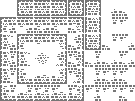
\includegraphics{images/walls.png} 
    \caption{All possible wall textures used in the prototype}
    \label{figure:walls}
\end{figure}

I decided to use a style that, in addition to visualizing the edge, also includes unique details inside the wall, depending on orientation, shape, and width. To achieve this style, there are exactly 48 possible wall shapes and orientations to choose from, shown in figure \ref{figure:walls}.

To retrieve the appropriate sprite from the tilemap, I first represented a tile's neighboring eight tiles as a bitmask, the greatest bit storing the value for the top-left neighbor, and following a reading order to store the others, the bottom-right neighbor being the last. Then I create a dictionary object, containing all the possible 256 in total bitmasks as keys, and the atlas coordinates (a two-dimensional vector representing a sprite's position inside the tileset) of their corresponding sprites. To make the process of filling up the dictionary slightly easier, I created patterns (similar to RegEx) consisting of eight nullable Booleans, describing the requirements for the bitmasks that correspond to the same sprite in the following way:

\begin{enumerate}
  \item If a bit must be 1 (wall), its value in the pattern is true
  \item If a bit must be 0 (empty), its value in the pattern is false
  \item If it does not matter whether a bit is 1 or 0, its value in the pattern is null
\end{enumerate}

Then I pass the patterns and the atlas coordinates of the desired sprite to a method that generates all possible bitmasks that match the pattern and adds them to the dictionary with the provided coordinates.

After the dungeon generation is finished, an additional pass is performed that is responsible for filling up the TileMapLayer with the adequate wall tiles, using the above-mentioned dictionary.

\subsection{Extraction points}

A defining part of extraction games are extraction points that players can use to leave the battlefield and return to a safe zone where they can manage the collected loot. In the prototype, ladders were used for such a purpose, which were randomly placed on the map. When the difficulty parameter was introduced, so was the minimum distance between the ladders, allowing them to be placed sparsely on higher difficulties.

